\chapter {Charakterystyka projektu}
\section {Uzasadnienie realizacji projektu}
Projekt realizowany jest w celu stworzenia aplikacji, która zostanie wdrożona do wirtualnego dziekanatu.
Dodanie nowej funkcji do wirtualnego dziekanatu ma usprawnić rekrutację na studia oraz dodawanie zdjęć.
\section {Nazwa projektu}
Aplikacja na system android - kadrowanie.
\section {Zakres projektu}
W projekcie zostanie wykonana aplikacja na system android, w której znajdzie się opcja kadrowania i przycinania zdjęć portretowych.
\section {Czas realizacji projektu}
\begin{itemize}
\item przygotowanie interfejsu aplikacji w języku Java,
\item wprowadzenie funkcji dodawania zdjęć, 
\item wprowadzenie funkcji podstawowego kadrowania zdjęć, 
\item wprowadzenie funkcji specjalistycznego kadrowania zdjęć z opcją ustalenia wymiarów.
\end{itemize}

\section{Plan realizacji projektu}
\begin{itemize}
\item [1.] 12.10.2016 Wyszukanie w Internecie kodu źródłowego aplikacji kadrującej.
\item [2.] 19.10.2016 Instalacja środowiska oraz potrzebnych składników do wirtualizacji telefonu z systemem Android na komputerze. 
\item [3.] 26.10.2016 Przygotowanie interfejsu aplikacji w środowisku programistycznym Android Studio:
\begin{itemize}
\item [a)] ekran powitalny aplikacji,
\item [b)] ekran z funkcją wczytywania zdjęć.
\end{itemize} 
\item [4.] 09.11.2016 Dodanie do aplikacji funkcji wczytywania i przycinania zdjęć.
\item [5.] 16.11.2016 Dodanie do aplikacji funkcji zapisywania zdjęć.

\end{itemize}

\subsection{Diagram następstwa produktów}
\subsection{Rezultaty i oddziaływanie}
Projekt będzie miał znaczący wpływ na usprawnienie oraz przyspieszenie przyjmowania kandydatów na studia. Zniknie problem ze zdjęciami w złym wymiarze oddawanymi przez kandydatów.


\section{Analiza interesariuszy}
Zlecający projekt ma na celu usprawnienie istniejące systemu uczelnianego rekrutacyjnego poprzez szybkie dodawanie odpowiednio skadrowanych zdjęć.


\section{Analiza instytucjonalna i techniczna}
\subsection{Wymogi prawne (i inne) związane z realizacją projektu}
\begin{itemize}
\item dobranie odpowiedniej licencji na program
\end{itemize}
\subsection{Struktura organizacyjna zarządzania projektem}
Osobami odpowiedzialnymi za kierowanie projektem są: Damian Pulit, Paweł Bodziony i Patryk Kubisz. \\
Do obowiązków lidera należy m.in.:
\begin{itemize}
\item wyznaczanie obowiązków dla poszczególnych członków zespołu,
\item nadzorowanie pracy poszczególnych członków zespołu,
\item planowanie, a następnie kierowanie realizacją projektu według określonych działań i terminów, 
\item kontrolowanie przebiegu projektu i ewentualne jego korygowanie,
\item motywowanie zespołu,
\item konsultowanie wymagań dotyczących projektu ze zleceniodawcą.
\end{itemize}
Do obowiązków członków zespołu należą:
\begin{itemize}
\item wykonywanie poleceń lidera,
\item wykonywanie zgodnie z harmonogramem poszczególnych etapów projektu.
\end{itemize}
\subsection{Zasoby niezbędne do realizacji projektu}
\begin{itemize}
\item [a)] ludzkie: umiejętności programistyczne w języku Java, umiejętność pracy ze środowiskiem Eclipse, nabycie wiedzy związanej z tworzeniem aplikacji na system Android,
\item [b)] materialne: telefon z system z Android, kompilator Eclipse, jednostka stacjonarna lub mobilna PC, dostęp do Internetu.
\end{itemize}

\section{Analiza techniczna}
\subsection{Opis przyjętych rozwiązań technicznych}
\begin{itemize}
\item Instalacja środowiska programistycznego aplikacji mobilnych Android Studio.

\begin{figure}[h!]
\centering
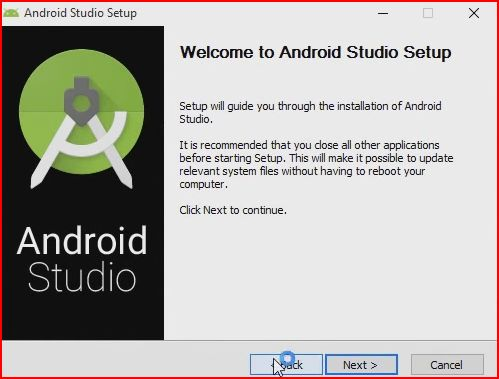
\includegraphics[width=0.5\linewidth]{fig/i1}
\caption{}
\label{fig:11}
\end{figure}

\begin{figure}[h!]
\centering
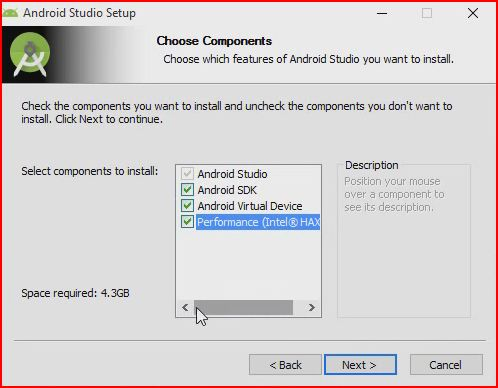
\includegraphics[width=0.5\linewidth]{fig/i2}
\caption{}
\label{fig:11}
\end{figure}

\begin{figure}[h!]
\centering
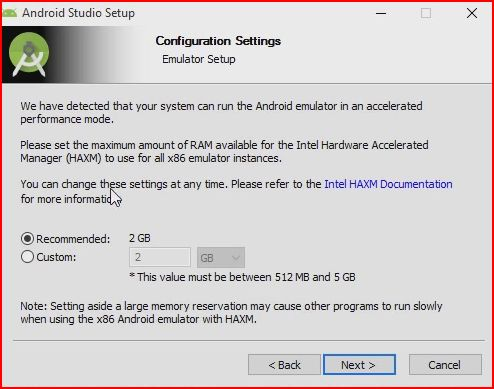
\includegraphics[width=0.5\linewidth]{fig/i3}
\caption{}
\label{fig:11}
\end{figure}

\begin{figure}[h!]
\centering
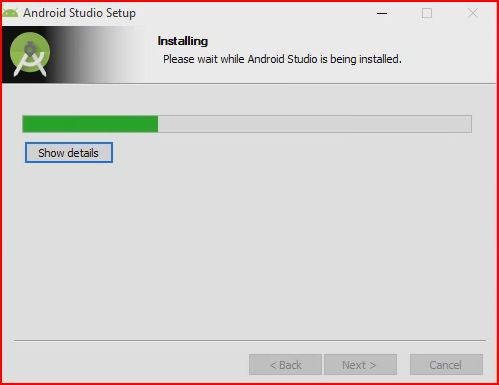
\includegraphics[width=0.5\linewidth]{fig/i4}
\caption{}
\label{fig:11}
\end{figure}

\begin{figure}[h!]
\centering
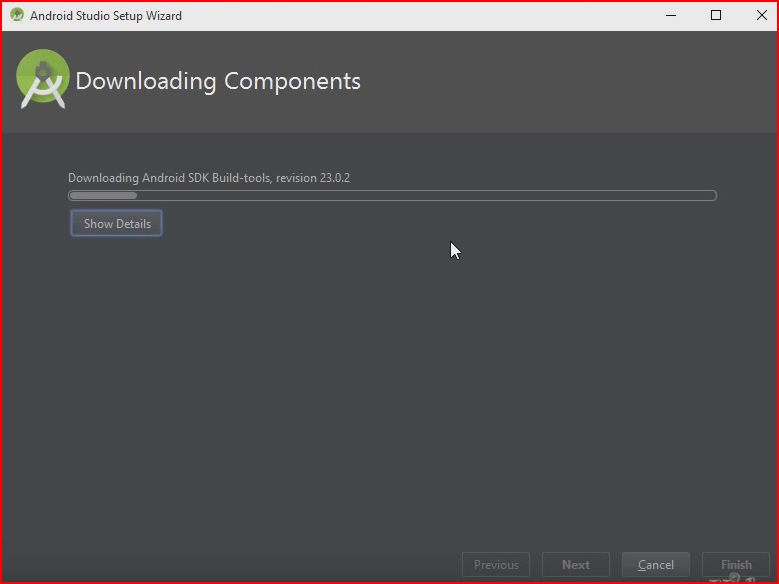
\includegraphics[width=0.5\linewidth]{fig/i5}
\caption{}
\label{fig:11}
\end{figure}

\begin{figure}[h!]
\centering
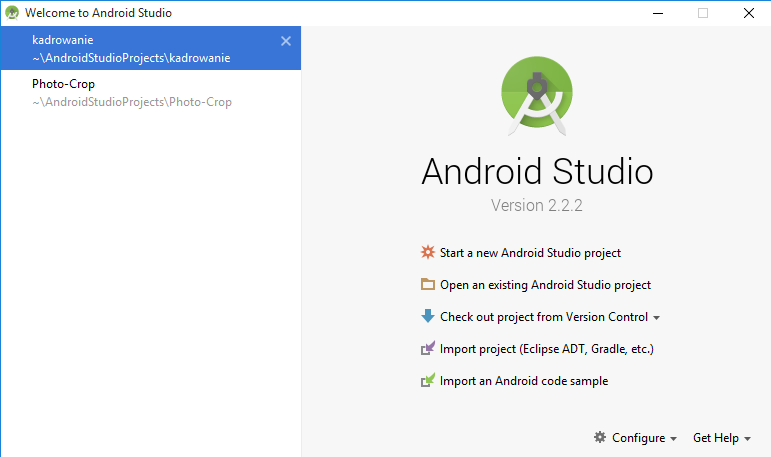
\includegraphics[width=0.7\linewidth]{fig/i6}
\caption{}
\label{fig:11}
\end{figure}


\clearpage
\item Praca w środowisku Android Studio.

\begin{figure}[h!]
\centering
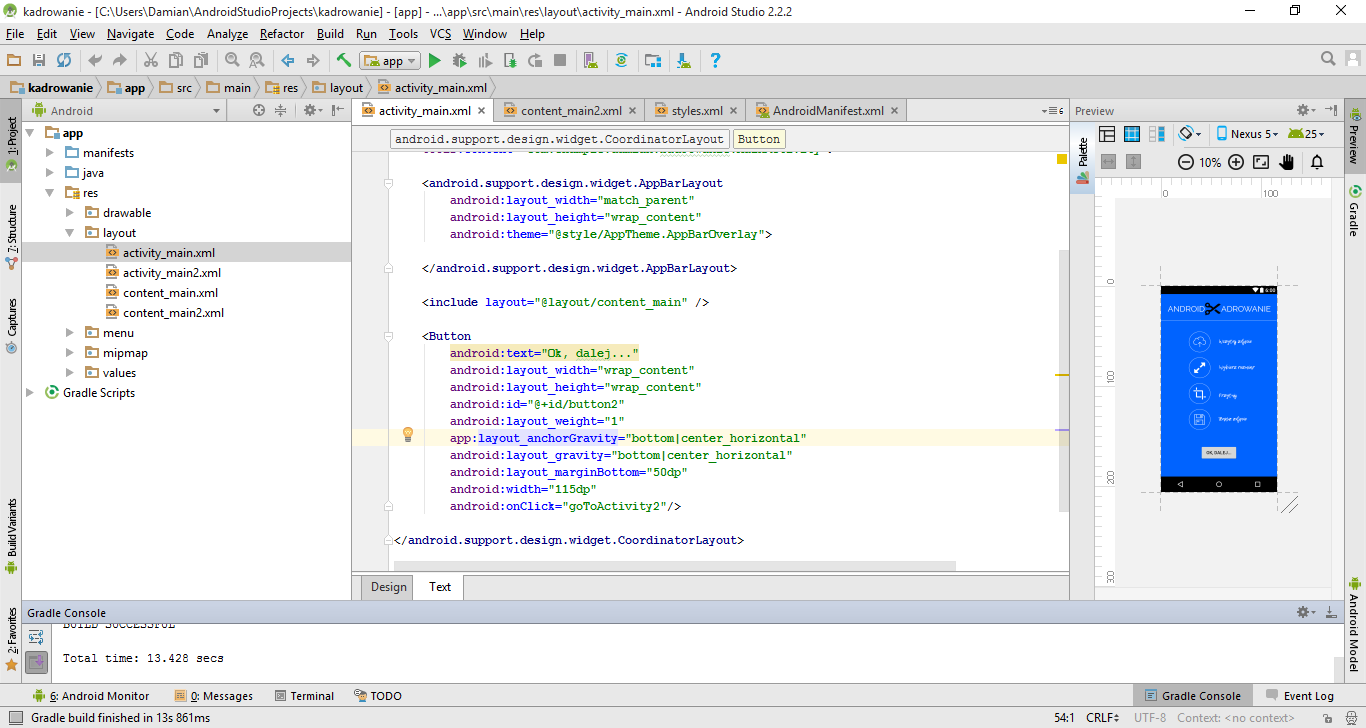
\includegraphics[width=0.9\linewidth]{fig/p1}
\caption{}
\label{fig:11}
\end{figure}


\item Uruchomienie aplikacji na emulatorze.


\begin{figure}[h!]
\centering
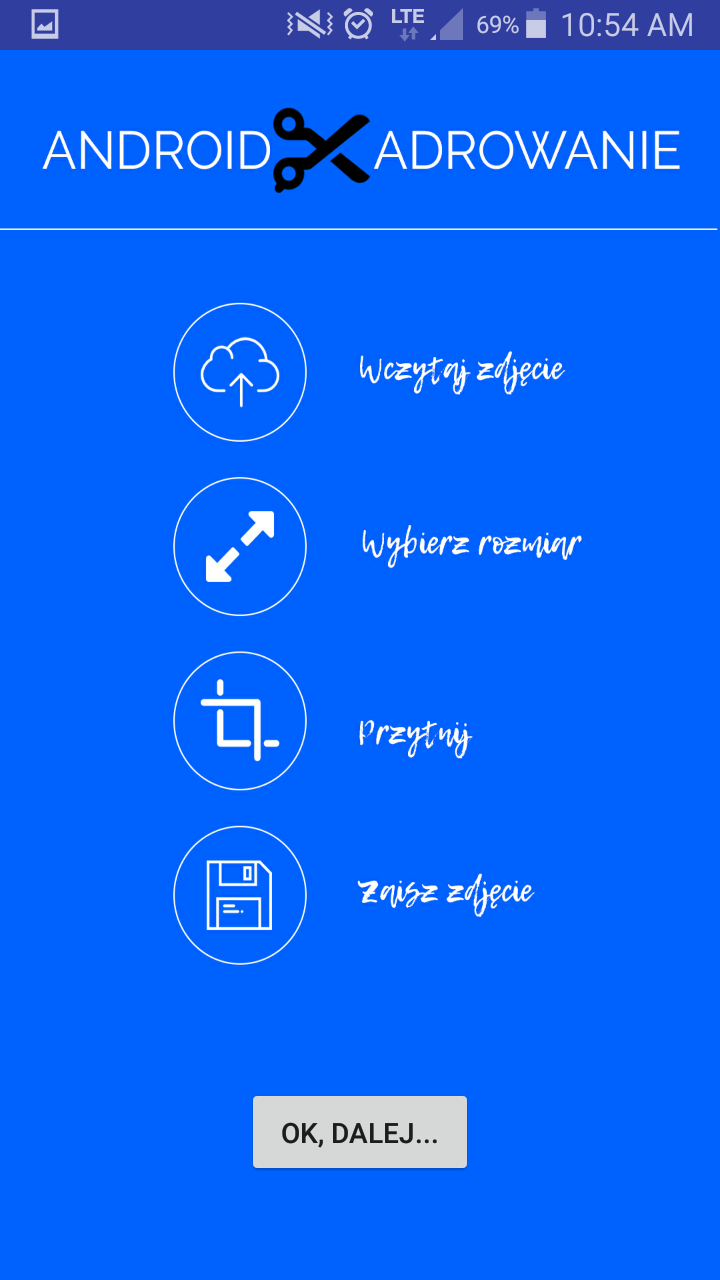
\includegraphics[width=0.3\linewidth]{fig/11}
\caption{Ekran powitalny}
\label{fig:11}
\end{figure}

\begin{figure}[h!]
\centering
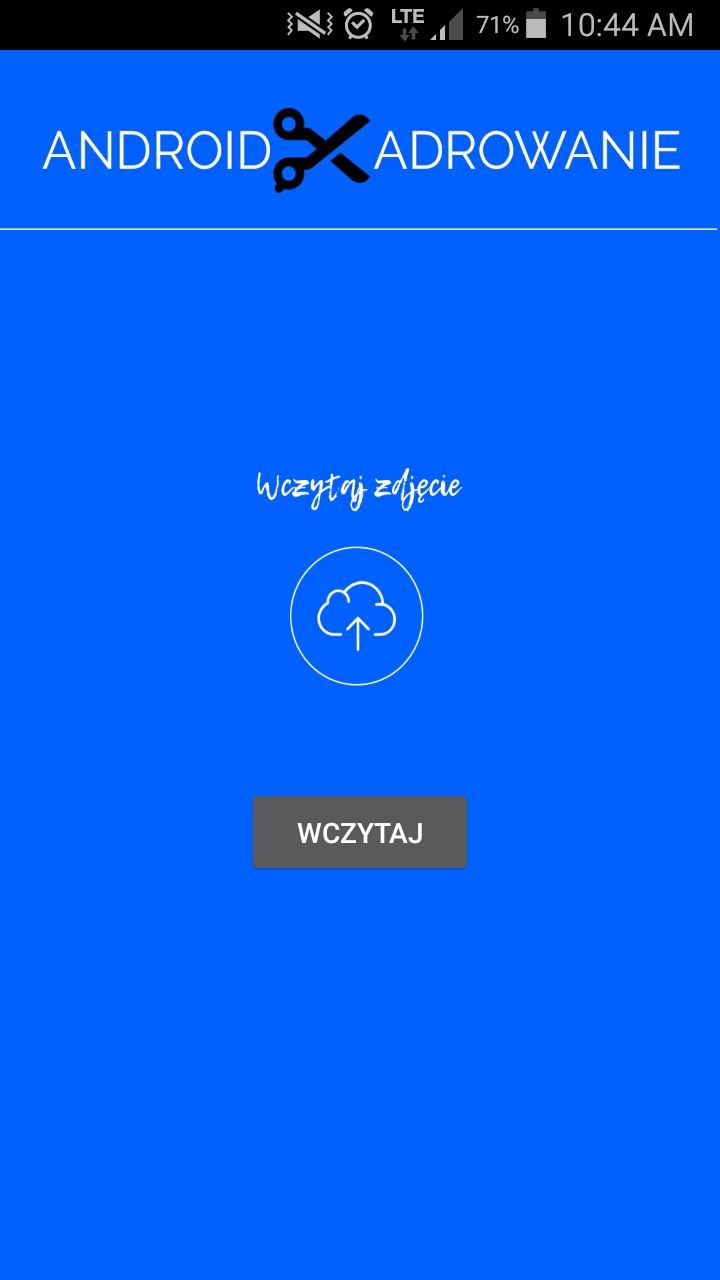
\includegraphics[width=0.3\linewidth]{fig/22}
\caption{Ekran wczytywania zdjęć}
\label{fig:11}
\end{figure}

\begin{figure}[h!]
\centering
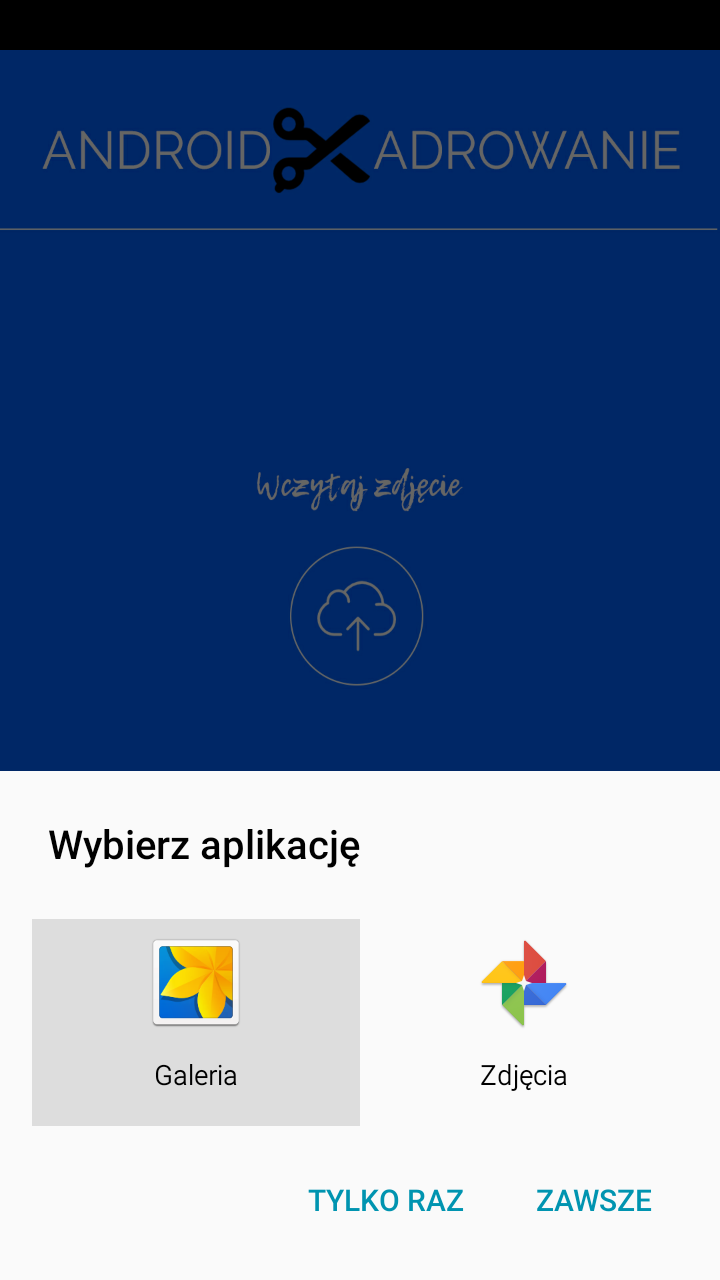
\includegraphics[width=0.3\linewidth]{fig/33}
\caption{Wybranie źródła zdjęcia do kadrowania}
\label{fig:11}
\end{figure}

\begin{figure}[h!]
\centering
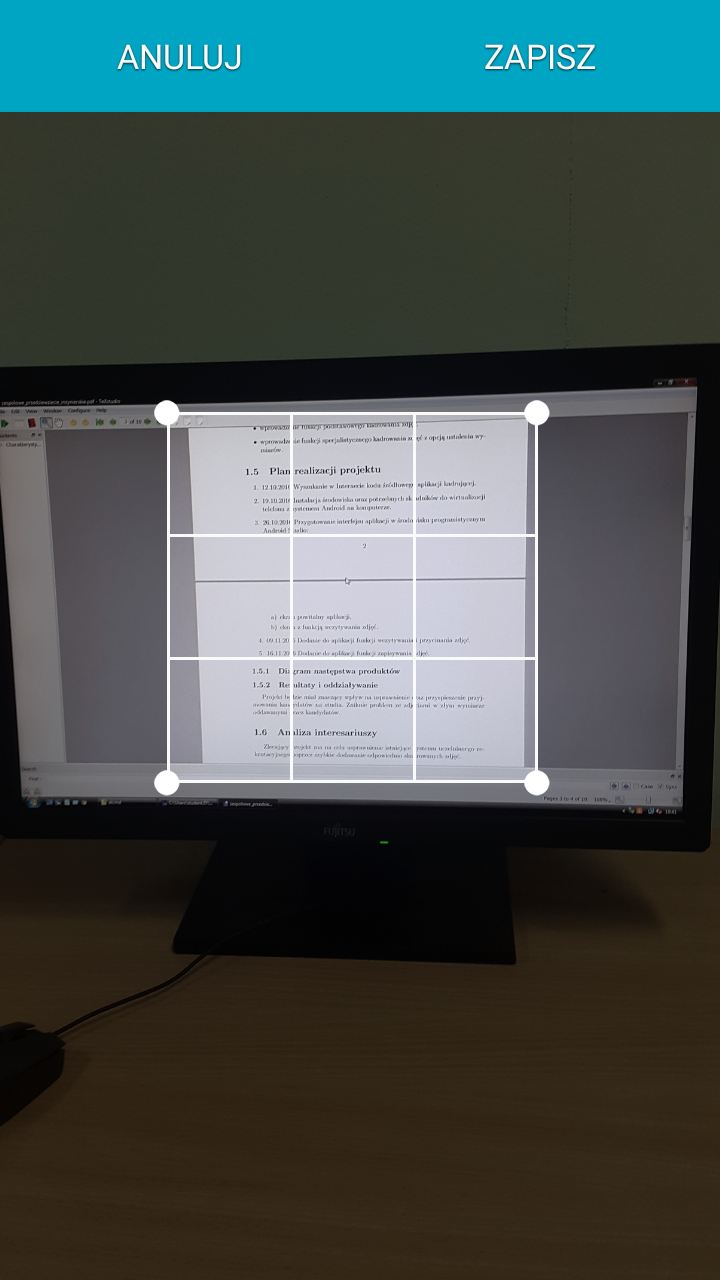
\includegraphics[width=0.3\linewidth]{fig/44}
\caption{Proces kadrowania}
\label{fig:11}
\end{figure}

\end{itemize}

\clearpage

\section{Instalacja aplikacji Image Cropper Quick Start na telefonie z system Android}
Ze strony https://android-arsenal.com/details/1/3487 należy pobrać plik apk na telefon, następnie odznaczyć opcję instalowania aplikacji z nieznanych źródeł, później za pomocą ściągniętego pliku apk instalujemy aplikację. 

\subsection{Analiza kodu źródłowego aplikacji}



